\documentclass[10pt, a4paper]{article}
% ===== Essential Packages =====
\usepackage[utf8]{inputenc}       % UTF-8 encoding
\usepackage[T1]{fontenc}          % Better font encoding
\usepackage{lmodern}              % Modern Latin Modern font
\usepackage{ctex}                 % Chinese support (must be loaded after fontenc)

% ===== Math & Symbols =====
\usepackage{amsmath}              % Advanced math
\usepackage{amssymb}              % Additional math symbols
\usepackage{mathrsfs}             % Ralph Smith's Formal Script
\usepackage{braket}               % Dirac bra-ket notation

% ===== Graphics & Tables =====
\usepackage{graphicx}             % Image support
\usepackage{float}                % Better float control
\usepackage{wrapfig}              % Wrapped figures
\usepackage{tikz}                 % Vector graphics
\usepackage[table]{xcolor}        % Colored tables
\usepackage{array}                % Enhanced tables
\usepackage{multirow}             % Multirow tables
\usepackage{tabularx}             % Adjustable-width tables
\usepackage{booktabs}             % Professional table lines
\usepackage{siunitx}              % SI units in tables
\usepackage{caption}              % Better captions
\usepackage{adjustbox}            % Box resizing

% ===== Code Listings =====
\usepackage{listings}             % Code blocks
\usepackage{tcolorbox}            % Colored boxes
\tcbuselibrary{listings, breakable} % Listings in tcolorbox

% ===== Misc =====
\usepackage{lipsum}               % Dummy text
\usepackage{footmisc}             % Better footnotes
\usepackage[margin=1in]{geometry} % Page margins
\title{牛顿环}
\author{张世航}
\begin{document}
	\maketitle
	\section{实验数据}
	\[\begin{tabular}{|c|c|c|c|c|c|c|c|c|}
		\hline
		\text{环数:}k & 10 & 15 & 20 & 25 & 30 & 35 & 40 & 45 \\
		\hline
		\text{左读数:}$x_1/mm$ & 29.609 & 30.149 & 30.698 & 31.179 & 31.622 & 32.021 & 32.390 & 32.731 \\
		\hline
		\text{右读数:}$x_2/mm $& 23.931 & 23.285 & 22.765 & 22.288 & 21.856 & 21.480 & 21.085 & 20.750 \\
		\hline
		\text{差值:}$(x_1-x_2)/mm$ &5.678 & 6.864&  7.933&  8.891&  9.766& 10.541& 11.3& 11.981\\
		\hline
		\text{差值平方:}$(x_1-x_2)^2/mm^2 $&32.24  &47.11&  62.93 & 79.05  &95.37& 111.11 &127.8 &143.54\\
		\hline
	\end{tabular}\]
	\section{最小二乘法}
	
	
	\begin{figure}[H]
		\centering
		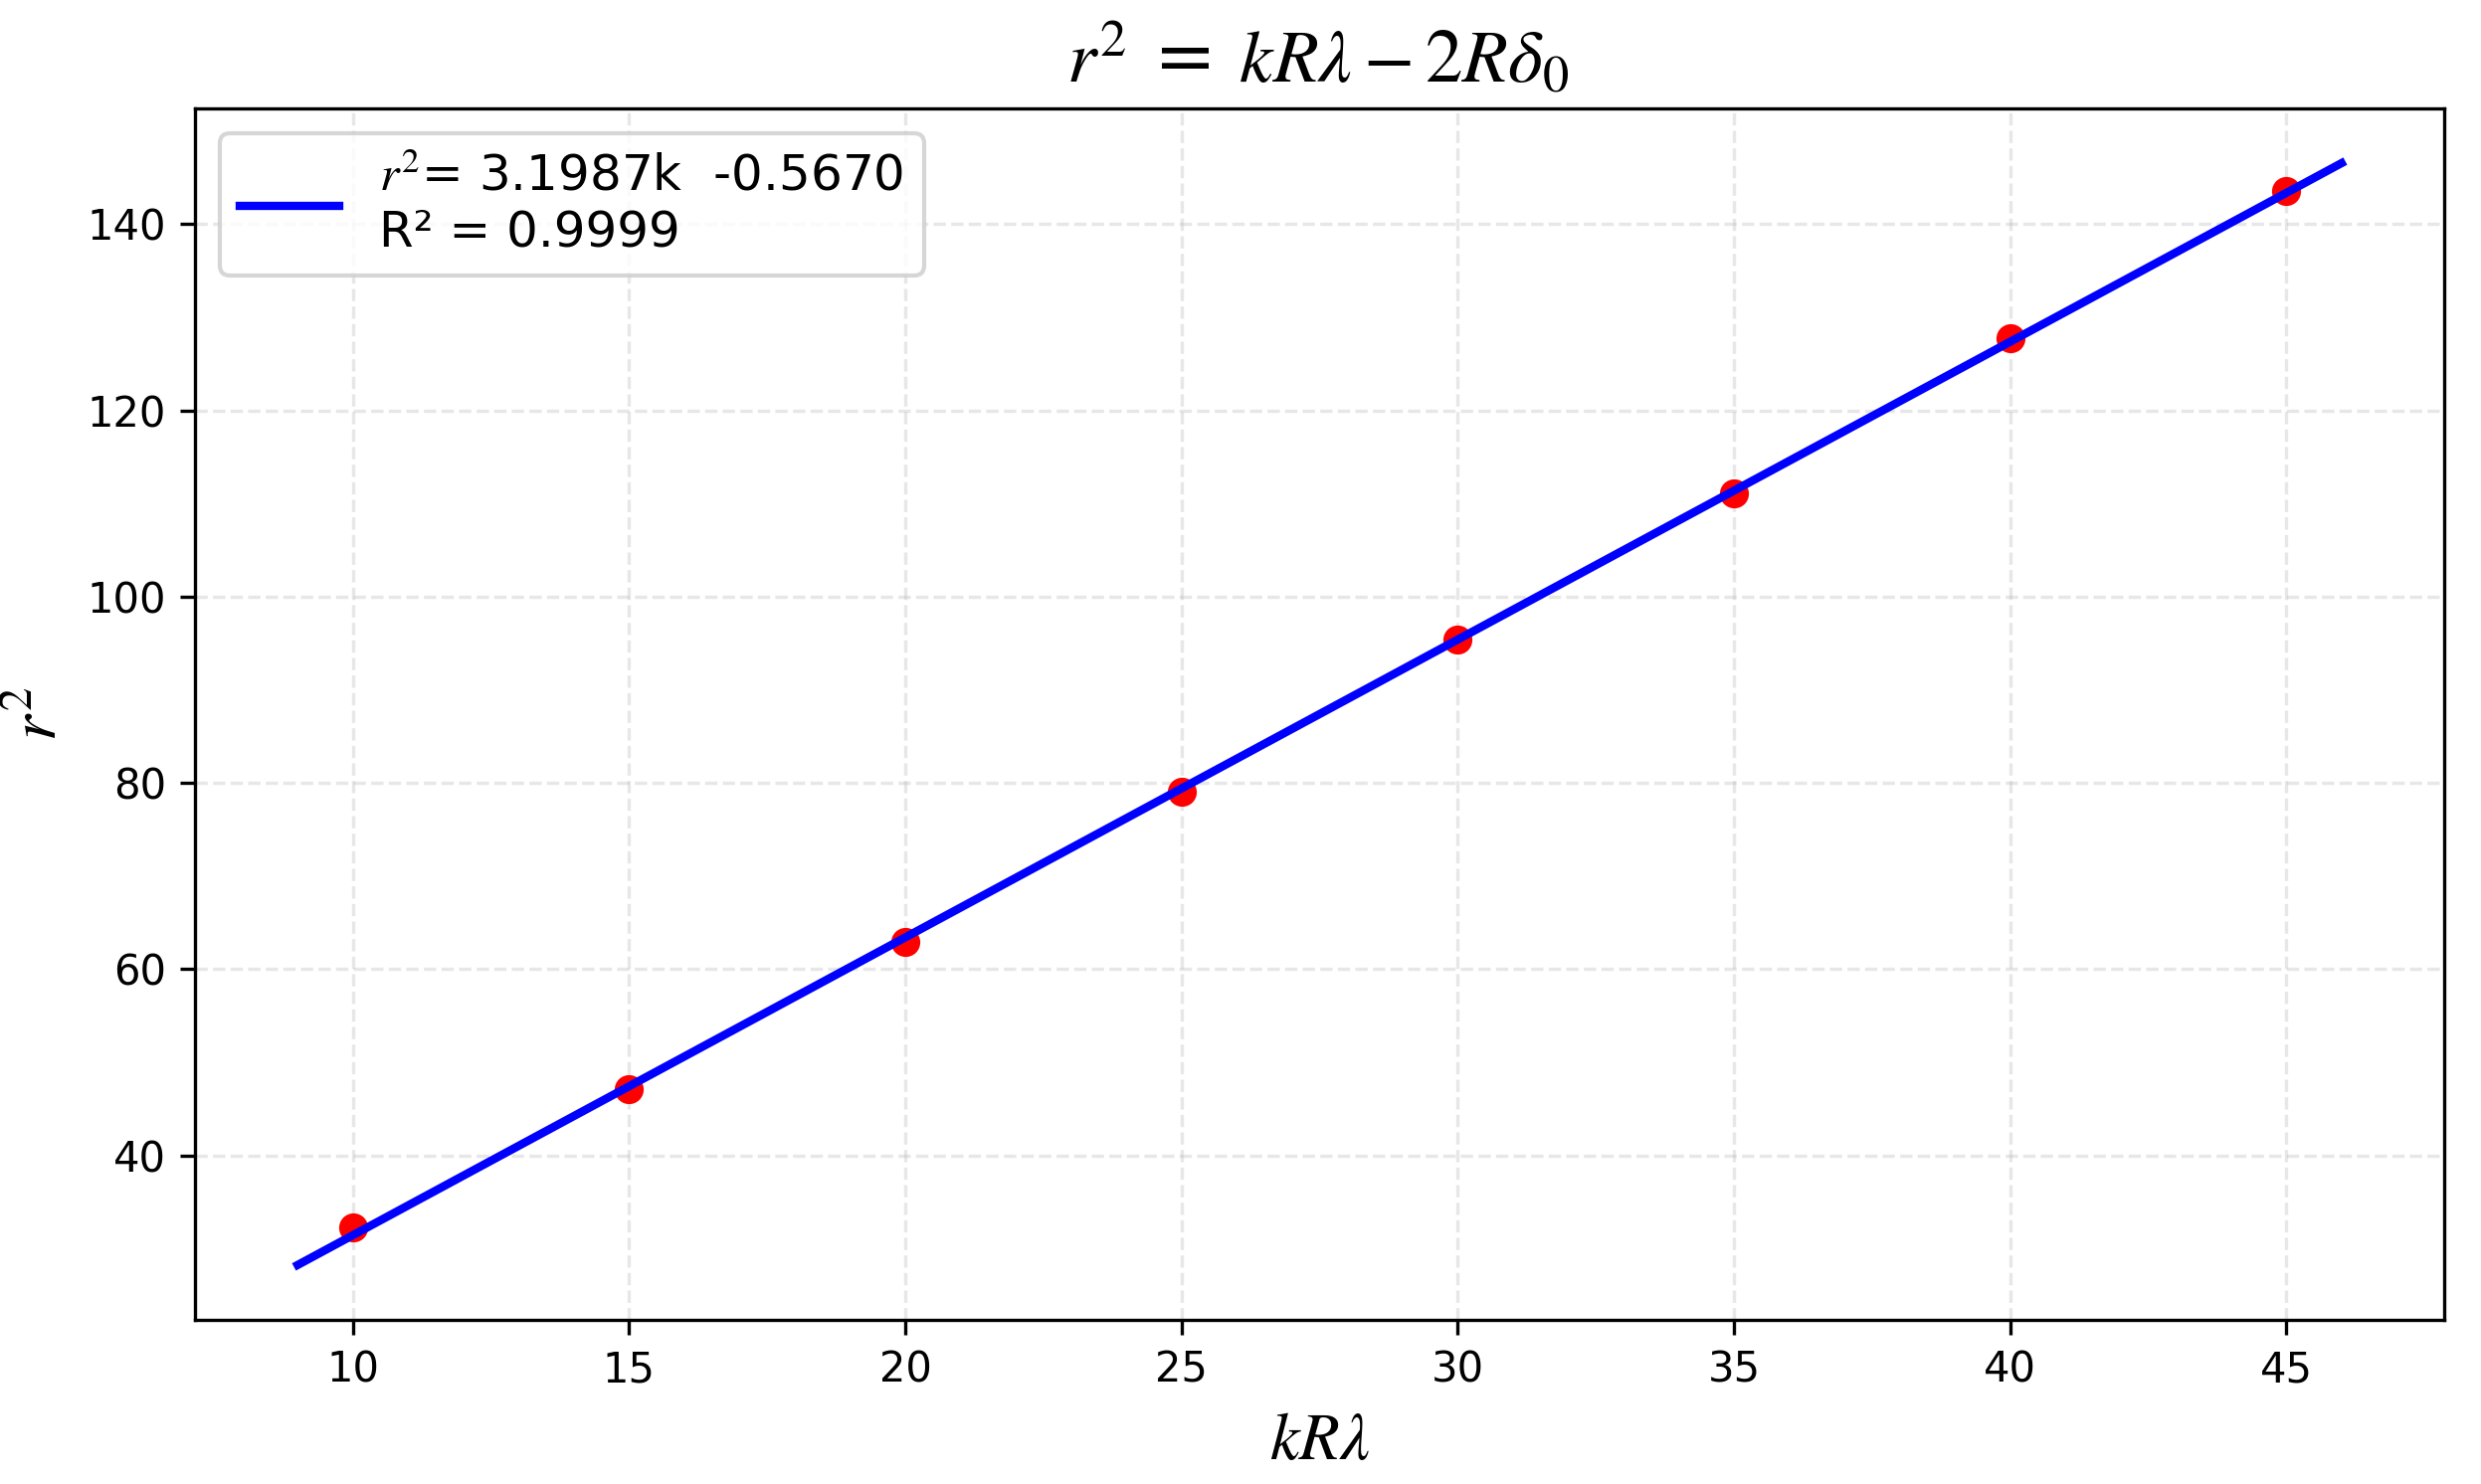
\includegraphics[width=0.7\linewidth]{1}
		\caption{最小二乘法}
		\label{fig:1}
	\end{figure}
	
	注意,这里的$r^2$指的是圆环直径的平方,所以要$r^2=4R_{\text{圆环}}^2$
	\[\begin{cases}
		\text{斜率}:3.198668654761905\\
		\text{截距}:-0.5669663809523939\\
		R^2\text{值}:0.9998704236040188\\
	\end{cases}\]
	 我们知道了斜率$k_1 = 3.198668654761905$,则\[R = \frac{k_1}{4\times\lambda}\times10^{-6} = \frac{3.198668654761905}{589.3\times 10^{-9}\times4}\times10^{-6}m=1.3569780480069173m\]
	 
	 \section{逐差法}
	 \[Y_1 = D_{45}^2-D_{25}^2 = 64.49448000000007mm^2\]
	 \[Y_2 = D_{40}^2-D_{20}^2 = 64.87053599999999mm^2\]
	 \[Y_3 = D_{35}^2-D_{15}^2 = 63.998185mm^2\]
	 \[Y_4 = D_{30}^2-D_{10}^2 = 63.13507199999995mm^2\]
	 
	 \[R_1 = \frac{Y_1}{\lambda\times20\times4} = 1.3680315628712043m\]
	 \[R_2 = \frac{Y_2}{\lambda\times20\times4} = 1.3760083149499405m\]
	 \[R_3 = \frac{Y_3}{\lambda\times20\times4} = 1.3575043483794331m\]
	 \[R_4 = \frac{Y_4}{\lambda\times20\times4} = 1.3391963346343108m\]
	 
	 \[R = \frac{R_1+R_2+R_3+R_4}{4}=1.3601851402087222m\]
	 
	 \section{误差分析}
	 \subsection{最小二乘法的误差分析}
	 由于我们只进行了一次的测量,所以没有A类不确定度.\\
	 我们的螺旋测微器的极限为$0.01mm$,则\[\Delta_{R}  =2.449305401279594\times10^{-3}m
	  \]
	 则 \[R = (1.3569780480069173\pm2.449305401279594\times10^{-3})m\]
	 
	 \subsection{逐差法的误差分析}
	 \[\mu(D_k) = \frac{1\times10^{-5}}{\sqrt{3}}m = 5.7735\times10^{-6}m\]
	 \[\mu(R)=\sqrt{\sum_k(\frac{\partial R}{\partial D_k}\times\mu(D_k))^2}=\frac{\mu(D_k)}{160\lambda}\sqrt{\sum_k D_k^2}=1.6191033280672995\times10^{-3}m\]
	 则\[R =\frac{R_1+R_2+R_3+R_4}{4}=(1.3601851402087222\pm1.6191033280672995\times10^{-3})m\]
\end{document}